% CS670 - Reinforcement Learning
% Dynamic Programming Assignment
% Gabriel Dulac-Arnold <gabe@squirrelsoup.net>
% Johannes H. Jensen <johannj@stud.ntnu.no>
\documentclass[a4paper]{article}
%\usepackage{multicol}
\usepackage{graphicx}
\usepackage[top=2cm,nohead,nofoot]{geometry}

\author{Gabriel Dulac-Arnold $<$gabe@squirrelsoup.net$>$ (CS09F004) \\
Johannes H. Jensen $<$johannj@stud.ntnu.no$>$ (CS09F005)}
\title{CS670 - Reinforcement Learning \\
\emph{Dynamic Programming Assignment}}

\begin{document}
\setlength{\parskip}{2ex}
\maketitle

\section{Value Iteration}

Running value iteration $\theta=0.01$ produced the following value functions:

\begin{figure}[h]
\center
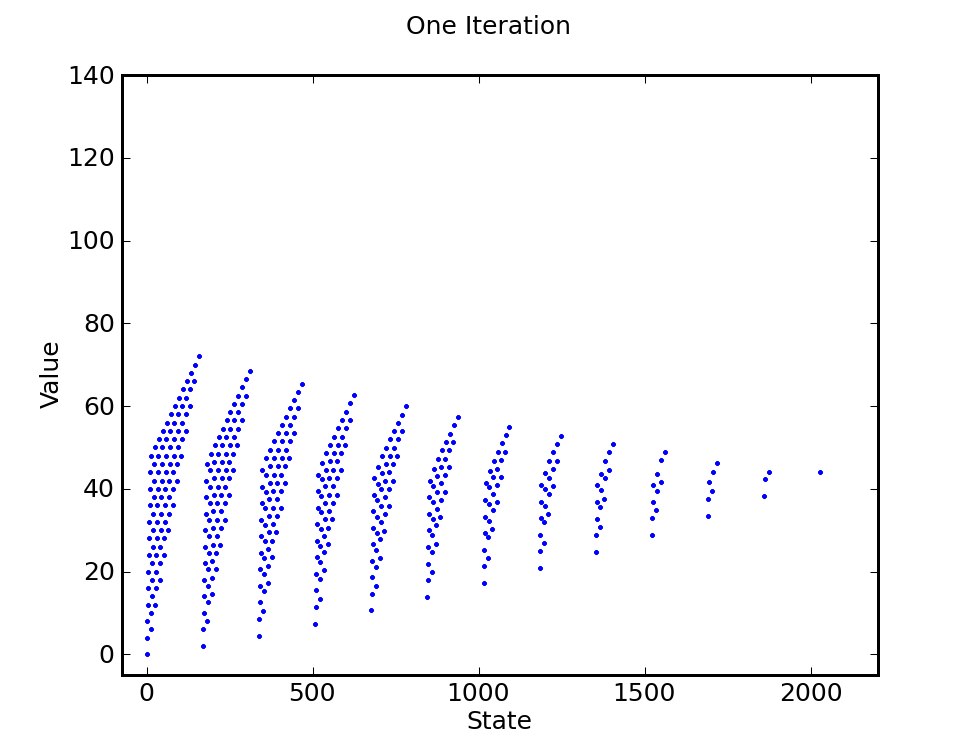
\includegraphics[scale=0.75]{../graphs/value_iteration/one_iteration.png}
\caption{$V(s)$ after sweep 1}
\end{figure}

\begin{figure}[h]
\center
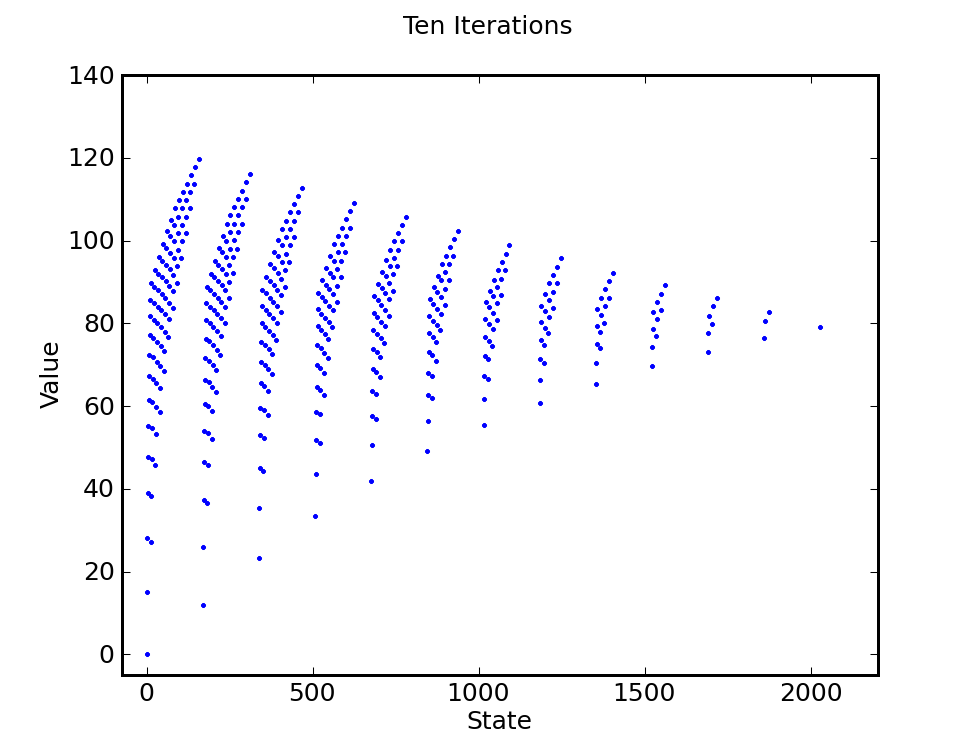
\includegraphics[scale=0.75]{../graphs/value_iteration/ten_iterations.png}
\caption{$V(s)$ after sweep 10}
\end{figure}

\begin{figure}[h]
\center
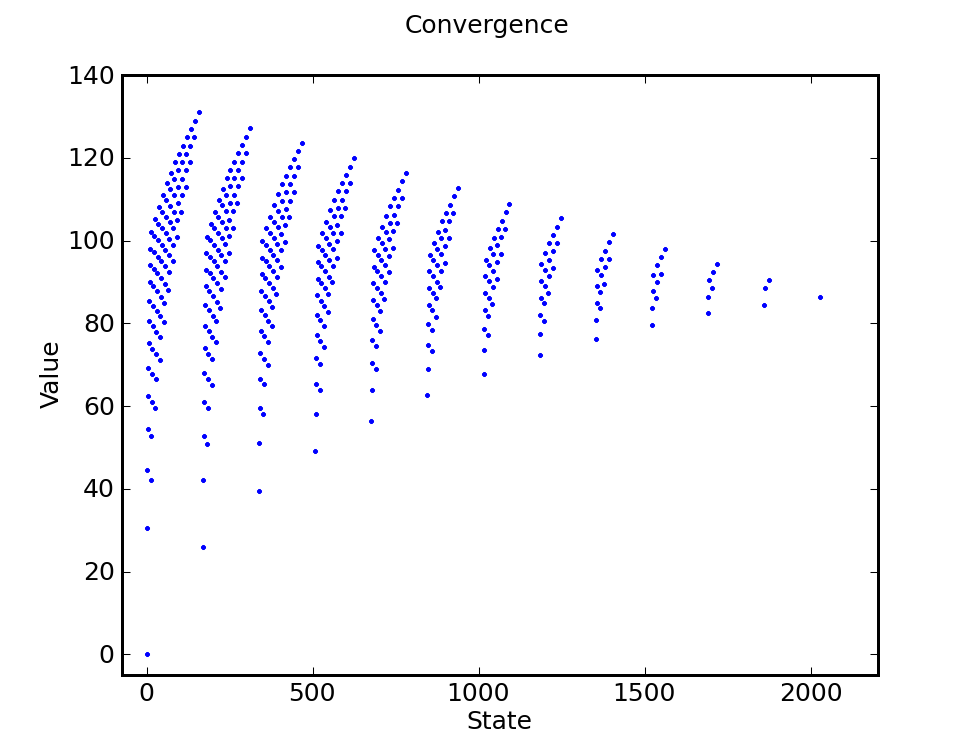
\includegraphics[scale=0.75]{../graphs/value_iteration/convergence.png}
\caption{$V*(s)$ at convergence}
\end{figure}

\end{document}

